\documentclass{eepecan}

% separate authors with \and 

\author{Cesar Luis Aybar Camacho %\and 
	%Surname Name \and 
	%Surname Name \and 
	%Surname Name \and 
}

\title{eePEcAn}
\subtitle{Integrating Google Earth Engine with the PEcAn project}

%\documentType{Preprint (submitted version)}
%\documentType{Postprint (	|accepted version)}
%\documentType{Article}
%\documentType{Working Paper}
%\documentType{Version of Record}


%\versionAvailableAtDOI{10....}
%\versionAvailableAtURN{urn:nbn:de:kobv:1234}
%\versionAvailableAtRefubium{fub188/12345}
\versionAvailableAt{\URL{https://github.com/csaybar/eePEcAn}}


%\citationDetails{}


\yearOfPublication{2020}


%\termsOfUse{\AllRightsReserved}
%\termsOfUse{\CCBY}
%\termsOfUse{\CCBYSA}
%\termsOfUse{\CCBYND}
%\termsOfUse{\CCBYNC}
%\termsOfUse{\CCBYNCSA}
\termsOfUse{\apache}
%\termsOfUse{Example \URL{http://www.###.org} more text}

%\publisherPhrase{This is the peer reviewed version of the above mentioned article. This article may be used for non-commercial purposes in accordance with publisher policy for use of self-archived versions.}
\renewcommand\thesection{\arabic{section}}

\begin{document}    
	\charitetitle
	\section{Introduction}
	\subsection{What is PEcAn?}
	Ecosystem models are essential for the development of scientific and operational applications, which allow to understand the terrestrial biosphere and, for instance, forecasting changes in the carbon cycle and its impact on natural and human systems. The amount of data being collected and produced is increasing on daily basis as we enter the "big data" era, but only a fraction of this data is being used to constrain models (Cowdery, et. al, 2018). Predictive Ecosystem Analyzer (PEcAn) is a framework, which is developed mainly in R, for ecosystem modeling that offers researches the opportunity to create 100\% reproducible and transparent data analysis pipelines. Currently,  PEcAn is comprised of:
	\begin{itemize}
	\item An application program interface (API) that provides a friendly-user I/0 interface to interact with 11 different ecosystem models.
 	\item An uncertainties data analysis module.
	web-based user interface and visualization tools (that use shiny).
	\item An extensible collection of modules to handle specific types of analyses, model-data syntheses, and data processing.
	\end{itemize}

	\begin{novspacecenter}
		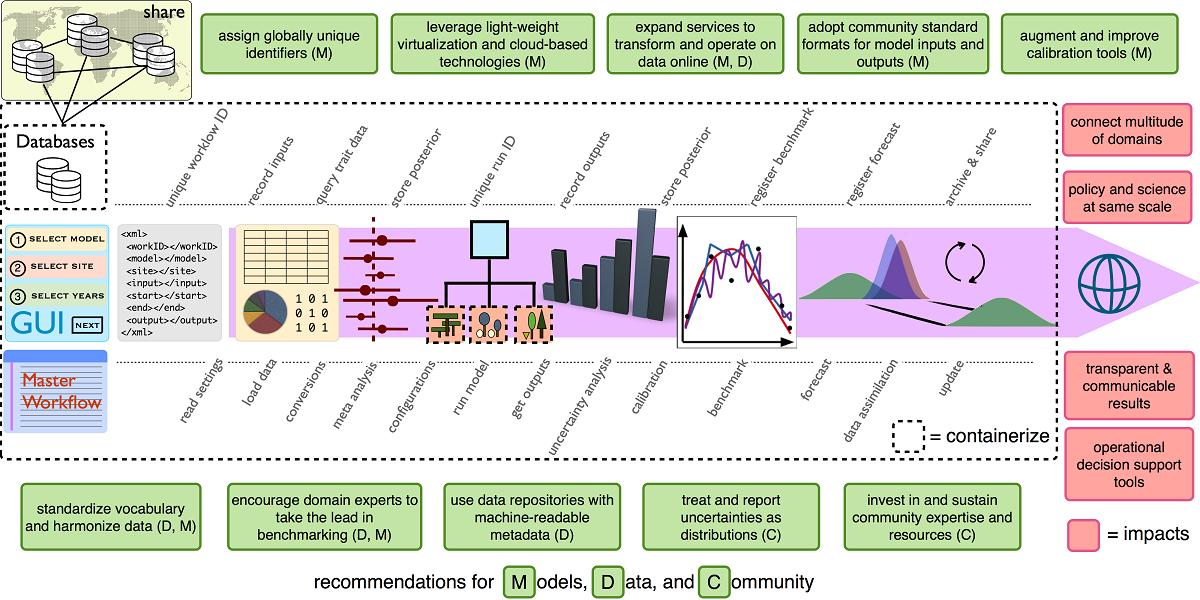
\includegraphics[width=160mm]{figures/fig01_main}
		\label{fig:fig01main}
	\end{novspacecenter}
	\subsection{How run PEcAn?}
	There are three principal ways to install PeCAN in a system.
	\begin{itemize}
		\item Virtual machine
		\item PEcAn Docker
		\item PEcAn OS specific installation
	\end{itemize}

	The most intuitive and user-friendly form to install PEcAn is using docker. All you have to do is create a \emph{docker-compose.yml}
	file, adapt it according to the 	\href{https://pecanproject.github.io/pecan-documentation/master/pecan-manual-setup.html}{documentation}, and then run:
	
	\begin{lstlisting}
		docker-compose -p pecan up -d
	\end{lstlisting}

	
	\begin{novspacecenter}
	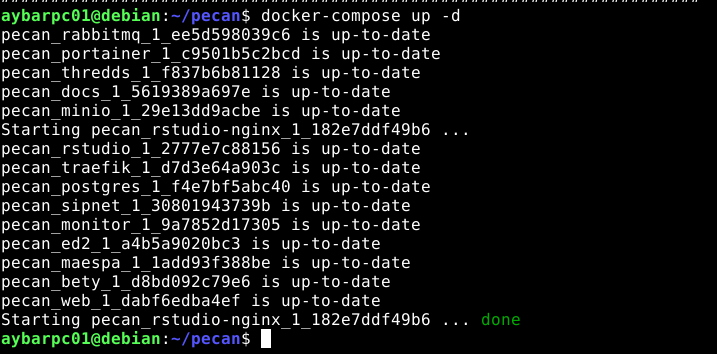
\includegraphics[width=120mm]{figures/fig02_docker}
	\label{fig:fig01main}
	\end{novspacecenter}


	If all of the containers started successfully, you should be able to access the various components from a browser via the following URLs (if you run these commands on a remote machine replace localhost with the actual hostname).
	\begin{itemize}
	\item PEcAn web interface (running models) – \href{http://localhost:8000/pecan/}{http://localhost:8000/pecan/} (NOTE: The trailing backslash is necessary.)
	\item PEcAn documentation and home page – \href{http://localhost:8000/}{http://localhost:8000/}
 	\item BETY web interface – \href{http://localhost:8000/bety/}{http://localhost:8000/bety/}
	\item File browser (minio) – \href{http://localhost:8000/minio/}{http://localhost:8000/minio/}
	\item RabbitMQ management console (for managing queued processes) – \href{http://localhost:8000/rabbitmq/}{http://localhost:8000/rabbitmq/}
	\item Traefik, webserver showing maps from URLs onto their respective containers – \href{http://localhost:8000/traefik/}{http://localhost:8000/traefik/}
	\item Monitor, service that monitors models and shows all models that are online as well as how many instances are online and the number of jobs 	waiting. The output is in JSON – \href{http://localhost:8000/monitor/}{http://localhost:8000/monitor/}
	\end{itemize}

	\begin{novspacecenter}
	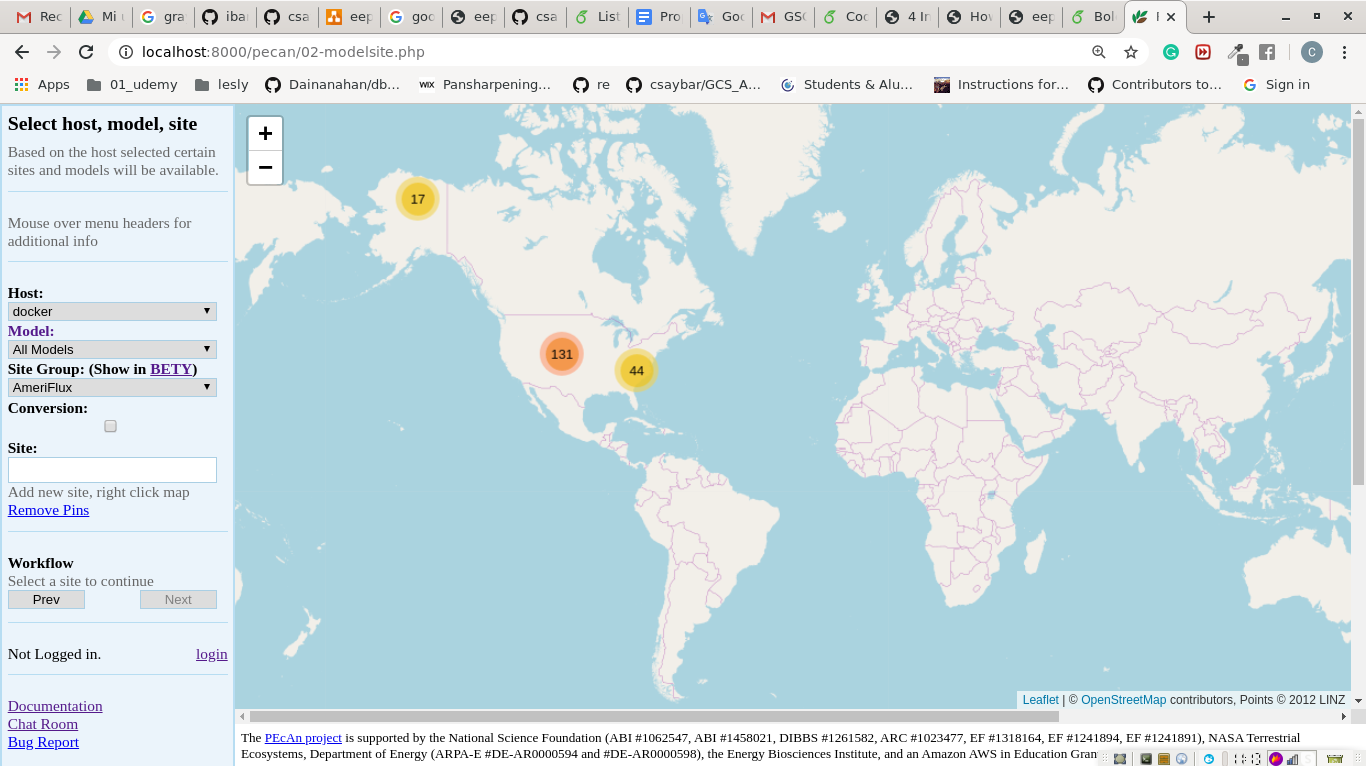
\includegraphics[width=150mm]{figures/fig03_lives}
	\label{fig:fig01main}
	\end{novspacecenter}

	\subsection{I/O PEcAn}
	The PEcAn system is configured using a XML file, often called \emph{pecan.xml}. You can find a complete list of all configurable parameters \href{https://pecanproject.github.io/pecan-documentation/master/pecanXML.html}{here}. The input data is used is used in \textbf{data assimilation, calibration and validation}. The principal parts of the PEcAn framework are:
	
	\begin{itemize}
	\item TRAIT -> Query the trait database for data and priors.
	\item META -> Run the PEcAn meta.analysis.
	\item CONFIG -> Write model specific configs.
	\item MODEL-> Start ecosystem model runs.
	\item OUTPUT ->	Get results of model runs.
	\item ENSEMBLE -> Run ensemble analysis on model output. 
	\item FINISHED -> Pecan workflow complete.
	\end{itemize}
	
	\section{GEE sync PEcAn - Project Idea}
	
	Establishing GEE and PEcAn communication. Google Earth Engine (GEE) is a cloud service that makes remote sensing data available for Earth System science. GEE has an API through which certain geopspatial analyses could be performed. We want to establish an efficient GEE-PEcAn link to ingest the outputs of such analyses into the PEcAn workflow seamlessly. PEcAn team will provide the initial example code that runs on the GEE servers, the GSoC participant will build the link that pulls the results from GEE to PEcAn, as well as submitting the code remotely to the GEE servers through the PEcAn workflow.
	
	\section{eePEcAn: Implementation plan}
	
	\textbf{eePecAn:} Module to Integrate Google Earth Engine and PecAn \newline
	
	\noindent eePecAn is a three-part project:
	
	
	\begin{enumerate}
		\item \textbf{Handling Authentication and Initialization using R:} Google Earth Engine currently does not support R, which is the main language in which PecAn is developed.  So the first step is to create a synchronization between the Earth Engine Python API and R. For this step will be used \textbf{reticulate} very similar to what we could see in
		\href{https://github.com/csaybar/rgee}{rgee} with the difference that all credentials will be previously encrypted and stored in the file \textbf{pecan.xml} (the user could change their credentials to preference) and then be reconfigured in the /config folder of your system as a JSON file.
		
		\item \textbf{Extract time series by points(eePecan\_extract)}: The second part looks for a robust module for obtaining time series. The idea is to improve and simplify the \textbf{ \href{https://csaybar.github.io/rgee/reference/ee_extract.html}{rgee::ee\_extract}} function so that it is not limited to only \href{https://developers.google.com/earth-engine/ic_info}{5000 elements per request}. In order to guarantee the efficiency and speed of the process. \textbf{eePecan\_extract} will be carried out using the module \href{https://developers.google.com/earth-engine/joins_intro}{ee.Join}. The function will return a data.frame and would be as follows:
		
		\begin{lstlisting}
			library(PEcAn.all)
			eePecan_extract(
				ImageCollection = "MODIS/006/MOD13A2",
				sf_geometry = my_points,
				startdate = "2000-01-01",
				lastdate = "200-12-31",
			)
		\end{lstlisting}
		
		In addition to the implementation, I will perform  several control quality functions for the most popular datasets (MODIS, Sentinel2, Landsat 8,7,5, etc.) along with different unit tests, in order to guarantee a proficient performance. \textbf{Just to be clear, with eePecan\_extract you would be able to extract values from any Earth Engine Images or ImageCollections such as, for instance, Landsat, MODIS, Sentinel, GPM, TRMM, terraclimate, etc.}
		
		
		\item {\textbf{Improvement of the shiny app to display PEcAn outputs}}: The last GSoC, Shuang Lu enhance the PEcAn shiny app to visualizing model output data alongside external data. I intend to give the user the possibility of adding external data only by adding the \textbf{GEE collection name, the band name and the correction scale}. With only these arguments the time series will appear automatically (the date range will be obtained from the file \textbf{eePEcAn.xml}).
		
		\begin{novspacecenter}
			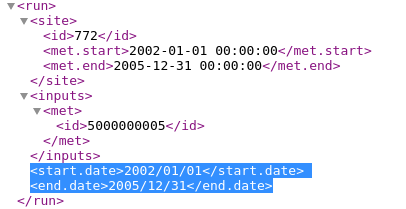
\includegraphics[width=80mm]{figures/fig04_xml}
			\label{fig:fig01main}
		\end{novspacecenter}
	\end{enumerate}
	\section{deliverables}
	\begin{itemize}
		\item An R module to authenticate and initialize the Earth Engine API. Full access to the API with the prefix ee\$…
		\item Implementing of the function eePecan\_extract to easily get time series using Google Earth Engine two approaches will be put into practice: using ee.Join and maps and filter.
		\item A series of functions to realize control quality to satellite images.
		\item Proper documentation and tests for the above-mentioned components.	
	\end{itemize}
	\section{Timeline}
	
	\subsection*{Before April 30:}
	
	\begin{itemize}
		\item To familiarize myself completely with the PEcAn infrastructure.
		\item Learn more about docker compose.
		\item Study more about PostgreSQL and how it is sync with docker.
	\end{itemize}
	
	\subsection*{April 30 – June 01 (Before the official coding time)}
	\begin{itemize}
		\item To do self coding to sync shiny and Google Earth Engine.
		\item During this period I will remain in constant touch with my mentor and the PEcAn community. I will remain active on slack and Mailing lists to discuss and finalize the modifications (if any) that need to be realized.
		\item With the help of my mentor, I will become absolutely clear about my future goals, the Earth Engine - PEcAn implementations that need to be done as well as the approach that I will follow to integrate my functions with the PEcAn project.
	\end{itemize}
	\subsection*{June 01 – June 29 (Official coding period starts)}
	\begin{itemize}
		\item Implementation of Authentication and Initialization of Google Earth Engine using R inside the PEcAn ecosystem.
		\item Implementation of \textbf{eePecan\_extract}.
		\item Testing of all my code using testthat.
	\end{itemize}			
	\subsection*{June 30 – August 10}
	\begin{itemize}
		\item Integration between \textbf{eePecan\_extract} and the shiny app to display PEcAn outputs.
		\item Test and document the existing code more thoroughly.
		\item Further refine tests and documentation for the whole project and PR.
	\end{itemize}			
	A buffer of two weeks has been kept for any unpredictable delay.

	\section{Personal details}	
	\textbf{Full Name:} Cesar Luis Aybar Camacho \newline \newline
	\textbf{Age:} 25 years \newline \newline
	\textbf{Sex:} Male \newline \newline
	\textbf{Study level:} Erasmus Graduate Student at the CDE program 2020-2022. \newline \newline
	\textbf{Why PEcAn?:} PEcAn is one of the few projects in Earth Science that is fully intended to be transparent and reproducible. I personally believe that the use of technology such as distributed version-control system, docker containers, and CI/CD are the right way for doing disruptive and high-impact science. I am definitely interested in learning from top-level researchers that use this stack on their daily basis. \newline \newline
	\textbf{Why this project?:} Google Earth Engine along with tensorflow are my favorite technologies. Although I spending more than a year learning about them, I have never used them in a tangible project with real results. I firmly believe that the GEE - PecAn project is the perfect opportunity to put everything I have learned into practice. \newline \newline

	\section{Stretch goals}
	\begin{itemize}
		\item Upload totally or partially the PostgreSQL database (BETYdb) to Google Earth Engine as a FeatureCollection. This would allow us generating, for instance, regional LAI analyzes quickly. 
		\item Automatically upload PEcAn output to Google Earth Engine using rgee. It would be helpful for sharing your results with other researchers.
		\item Automatically generation of documentation of Earth Engine functions and methods in the R style format: Currently this is implemented in rgee (\href{https://github.com/csaybar/rgee/blob/master/R/ee_help.R}{ee\_help}) but with several errors. It will be beneficial for both projects (rgee and eePEcAn) to have this function to quickly understand what each method or function of GEE does.
		\item Integrating the PEcAn project with \href{https://developers.planet.com/docs/data/}{Planet API}
	\end{itemize}
\end{document}

